\documentclass{article}
\usepackage{graphicx}
\usepackage{float}
\begin{document}
\begin{figure}[H]
\centering
\includegraphics[width=\textwidth]{thread-race_bar_chart.png}
\caption{Figure for thread-race}
\end{figure}

\begin{figure}[H]
\centering
\includegraphics[width=\textwidth]{thread-mutex-single_bar_chart.png}
\caption{Figure for thread-mutex-single}
\end{figure}

\begin{figure}[H]
\centering
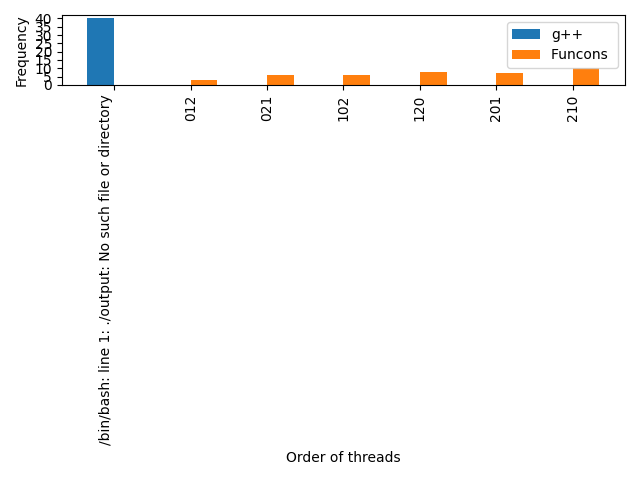
\includegraphics[width=\textwidth]{thread-race-with-sleep_bar_chart.png}
\caption{Figure for thread-race-with-sleep}
\end{figure}

\begin{figure}[H]
\centering
\includegraphics[width=\textwidth]{thread-mutex-multiple_bar_chart.png}
\caption{Figure for thread-mutex-multiple}
\end{figure}

\documentclass{standalone}
\usepackage{booktabs}
\usepackage[margin=1in]{geometry}
\usepackage{tabularx}
\usepackage{subcaption}
\begin{document}
\begin{center}
\caption{Summary of Test Differences}
\begin{tabularx}{\textwidth}{|X|X|X|X|}
\hline\hline
             Name &  Length of the program ($l$) &  Length of the permutated program ($\leq2l(l!)$) &  Number of Differences \\
\hline
shared\_mutex.cpp &                            4 &                                               66 &                     66 \\
        mutex.cpp &                            2 &                                                6 &                      0 \\
\hline\hline
\end{tabularx}
\subcaption{This table lists the number of differences in the test results. The The tests were run 2 times to ascertain the determinism. The number of tests that were rejected due to inconsistencies were 0.}\end{center}\end{document}
\begin{figure}[H]
\centering
\includegraphics[width=\textwidth]{condition_notify_scheduling_bar_chart.png}
\caption{Figure for condition_notify_scheduling}
\end{figure}


\end{document}